\documentclass{article}
\usepackage[utf8]{inputenc}
\usepackage{amsmath}
\usepackage{graphicx}
\usepackage{hyperref}
\usepackage{xcolor}
\usepackage[left=1in, right=1in]{geometry}
\usepackage{listings}
\usepackage{tikz}
\usetikzlibrary{positioning}

% Configure listings package for Python syntax highlighting
\definecolor{codegreen}{rgb}{0,0.6,0}
\definecolor{codegray}{rgb}{0.5,0.5,0.5}
\definecolor{codepurple}{rgb}{0.58,0,0.82}
\definecolor{backcolour}{rgb}{0.95,0.95,0.95}

\lstdefinestyle{pythonstyle}{
    backgroundcolor=\color{backcolour},   
    commentstyle=\color{codegreen},
    keywordstyle=\color{magenta},
    numberstyle=\tiny\color{codegray},
    stringstyle=\color{codepurple},
    basicstyle=\ttfamily\footnotesize,
    breakatwhitespace=false,         
    breaklines=true,                 
    captionpos=b,                    
    keepspaces=true,                 
    numbers=left,                    
    numbersep=5pt,                  
    showspaces=false,                
    showstringspaces=false,
    showtabs=false,                  
    tabsize=2,
    language=Python
}

\lstset{style=pythonstyle}

\title{Modelling in Biology Coursework II}
\author{Harsh Agrawal (CID\@: 02320622)}
\date{\today}

\begin{document}
\maketitle

\subsection*{Question 1}

\subsubsection*{a. Draw a graphical representation of the Markov Process describing the formation of a single channel, and give the associated rate matrix.}

\begin{figure}[htbp]
    \centering
    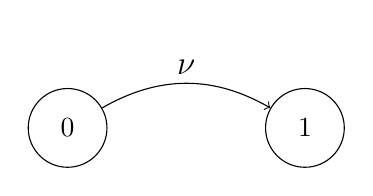
\begin{tikzpicture}[every node/.style={circle, draw, minimum size=1cm}, node distance=2cm]
        % Nodes
        \node (left) {0};
        \node (right) [right=of left] {1};

        % Arrow with rate
        \draw[->] (left) to[bend left] node[midway, above=-0.3cm, draw=none, font=\large, inner sep=1pt] {$\nu$} (right);
    \end{tikzpicture}
    \caption{\centering Markov Process for single channel formation from state 0 to 1 with transition rate $\nu$.}\label{fig:q1_process}
\end{figure}

The Rate Matrix of a Continuous Time Discrete State Markov Process is given by:

\[
    \mathbf{Q_{ij}} = \begin{pmatrix}
        K_{00} & K_{01} \\
        K_{10} & K_{11}
    \end{pmatrix}
\]

We know that $K_{01} = 0$ as state 1 is an absorbing state (the channel has
formed) and $K_{10} = \nu$ (rate of formation of channel). We can use these
values to fill the diagonal as the negative sum of the respective column.

\begin{equation}
    \boxed{\mathbf{Q_{ij}} = \begin{pmatrix}
            -\nu & 0 \\
            \nu  & 0
        \end{pmatrix}}
\end{equation}
\subsubsection*{b. Derive the probability $p_0(t)$ that the channel has not formed at time $t$}
To find the probability that the channel hasn't formed at time $t$, we first start with the evolution equation for the probability vector $\vec{p}(t)$.

\[
    \frac{d}{dt} \vec{p}(t) = \mathbf{Q} \cdot \vec{p}(t), \quad \text{where} \vec{p}(t) = \begin{pmatrix} p_{0}(t) \\ p_{1}(t) \end{pmatrix}
\]

We can further expand this to:

\[
    \frac{d}{dt} \begin{pmatrix} p_0(t) \\ p_1(t) \end{pmatrix} = \begin{pmatrix}
        -\nu & 0 \\
        \nu  & 0
    \end{pmatrix} \cdot \begin{pmatrix} p_{0}(t) \\ p_{1}(t) \end{pmatrix} = \begin{pmatrix} -\nu \cdot p_0(t) \\ \nu \cdot p_1(t) \end{pmatrix}
\]

Since we're only interested in $p_0(t)$, we obtain:

\[
    \frac{d}{dt} p_0(t) = -\nu \cdot p_0(t)
\]

We can solve this using the method of separation of variables.

\[
    \frac{dp_0(t)}{p_0(t)} \cdot \frac{1}{dt} = -\nu
\]

Integrating both sides, we get:

\[
    \int \frac{dp_0(t)}{p_0(t)} \cdot \frac{dt}{dt} = \int -\nu dt \implies \ln p_0(t) = -\nu t + C
\]

Exponentiating both sides, we get:
\[
    p_0(t) = e^{-\nu t + C}
\]

We have a known boundary condition at $t = 0$, $p_0(0) = 1$ (the probability of
the channel not being formed at time 0 is 1), so we can substitute this into
the equation to find $C$:
\[
    p_0(0) = e^{-\nu \cdot 0 + C} = e^C = 1 \implies C = 0
\]

This yields the final solution:
\begin{equation}
    \boxed{p_0(t) = e^{-\nu t}}
\end{equation}

\subsubsection*{c. What is the most likely time at which the channel forms?}

Since we already know that the time to form a channel is exponentially
distributed with the parameter $\nu$, we can use this to find the time where
the Probability Density Function is maximized.

\[
    f_{T}(t) = \nu e^{-\nu t}
\]

We can find the maximum by taking the derivative and setting it to 0. But we
can logically also see that at $t = 0$, $f_{T}(t) = \nu$. As $t$ increases, the
probability decreases as the function follows an exponential decay. Therefore,
without calculation, we can say that the maximum probability is at $t = 0$ and
thus the most likely time at which the channel forms is at:

\begin{equation}
    \boxed{t = 0}
\end{equation}

\newpage
\subsection*{Question 2}
\subsubsection*{a. Draw a graphical representation of the stochastic process $\mathbf{N(t)}$}
We have another Continuous Time Discrete State Markov Process with states $n = 0, 1, 2, \ldots, M$. This is a pure birth process (i.e, no transitions can occur from $n \rightarrow n-1$). Moreover, every transition occurs successively as $n \rightarrow n+1$ (i.e, no transitions can occur directly from $n \rightarrow n+2$).

\begin{itemize}
    \item At state $n = 0$, M channels can be formed independently with rate $\nu$. Thus
          \textit{the total rate of transition from $n = 0$ to $n = 1$ is $\nu \cdot M$.
              This makes intuitive sense as at $n=0$, transitions occur the fastest as any of
              the $M$ channels can form.}
    \item At state $n = 1$, $M-1$ channels are unformed and thus the total rate of
          transition from $n = 1$ to $n = 2$ is $ \nu \cdot (M-1)$. At state $n = M$, all
          $M$ channels are formed and thus this is an absorbing state.
    \item In general, at state $k$ for $k < M$, the rate of transition from $k
              \rightarrow k+1$ is $\nu \cdot (M-k)$
\end{itemize}

We can use this reasoning to draw the stochastic process as follows:

\begin{figure}[h]
    \centering
    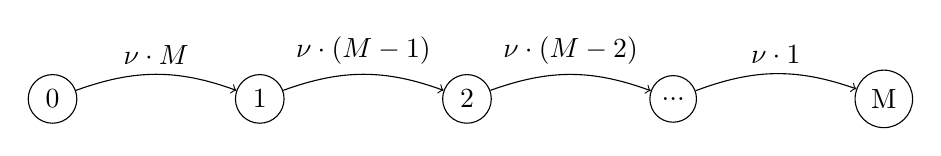
\begin{tikzpicture}[node distance=2cm, baseline=(current bounding box.center)] % Center the diagram
        % Define nodes for states 0, 1, 2, 3
        \node[circle, draw] (s0) {0};                % State 0
        \node[circle, draw, right=of s0] (s1) {1};   % State 1, positioned right of state 0
        \node[circle, draw, right=of s1] (s2) {2};   % State 2, positioned right of state 1
        \node[circle, draw, right=of s2] (s3) {...};   % State 3, positioned right of state 2
        \node[circle, draw, right=of s3] (s4) {M};

        % Draw curved arrows with transition rates
        \draw[->] (s0) to[bend left=20] node[midway, above] {$\nu \cdot M$} (s1); % From 0 to 1
        \draw[->] (s1) to[bend left=20] node[midway, above] {$\nu \cdot (M-1)$} (s2); % From 1 to 2
        \draw[->] (s2) to[bend left=20] node[midway, above] {$\nu \cdot (M-2)$} (s3); % From 2 to 3
        \draw[->] (s3) to[bend left=20] node[midway, above] {$\nu \cdot 1$} (s4); % From 3 to 4
    \end{tikzpicture}
    \caption{\centering Markov diagram for the stochastic process $\mathbf{N(t)}$.}\label{fig:q2_process}
\end{figure}

\subsubsection*{b. Explain why, for $0 \leq n \leq M$, we may write the following ODE for $p_n(t)$, the probability that $N = n$ at time $t$. Note that $p_n = 0$ for $n < 0$ or $n > M$ by definition.}

\[
    \frac{dp_n}{dt} = -\nu(M - n)p_n + \nu(M - (n - 1))p_{n-1}
\]

We start with the master equation for a generic Continuous Time Discrete State
Markov Process which states that the rate of change of the probability of being
in state $n$ is given by the sum of the incoming transitions to that state
minus the outgoing transitions from that state.

\[
    \frac{dp_n}{dt} = \sum_{m \ne n} p(n, t+dt \mid m, t) \cdot p(m, t) - \sum_{n \ne m} p(m, t+dt \mid n, t) \cdot p(n, t)
\]

For our condition, we know that there is a single incoming transition (from
$n-1$ to $n$) and a single outgoing transition (from $n$ to $n+1$). We can thus
simplify the incoming and outgoing transitions to:

\[
    \sum_{m \ne n} p(n, t+dt \mid m, t) \cdot p(m, t) = p(n, t \mid n-1, t) \cdot p(n-1, t) \quad \quad \text{\textcolor{gray}{(Incoming Transitions)}}
\]

\[
    \sum_{n \ne m} p(m, t+dt \mid n, t) \cdot p(n, t) = p(n + 1, t \mid n, t) \cdot p(n, t) \quad \quad \text{\textcolor{gray}{(Outgoing Transitions)}}
\]

Since we know the transition rates for going from $k \rightarrow k+1$ as $\nu
    \cdot (M-k)$, we can substitute these into the master equation to get:

\[
    p(n, t \mid n-1, t) \cdot p(n-1, t) = \nu(M-(n-1)) \cdot p_{n-1} \quad (k = n-1)
\]

\[
    p(n + 1, t \mid n, t) \cdot p(n, t) = \nu(M-n) \cdot p_n \quad (k = n)
\]

We can now substitute these into the master equation to get:

\begin{equation}
    \boxed{\frac{dp_n}{dt} = - \nu(M-n)p_n + \nu(M-(n-1))p_{n-1}}
\end{equation}

\subsubsection*{c. What is the stationary distribution $\mathbf{\pi_{n}}$ of the process?}
The stationary distribution $\pi_n$ is the long-term probability of being in state $n$ as $t \rightarrow \infty$. In a pure birth process, once all $M$ channels form, the system stays in state $M$ forever as it's an absorbing state.

As $t \rightarrow \infty$, the probability of being in state $n=M \rightarrow
    1$ (as all channels are formed). Since the probabilities in $\vec{\pi}$ must
sum to 1, we can say all other probabilities for $n \neq M \rightarrow 0$ at $t
    \rightarrow \infty$.

Therefore, the stationary distribution is:
\[
    \pi_n = \begin{cases}
        1 & \text{if } n = M \\
        0 & \text{otherwise}
    \end{cases}
\]
\subsubsection*{d. Using the `multiply and sum' technique, show that
    \[
        \frac{d}{dt}
        \langle N(t) \rangle = \nu(M - \langle N(t) \rangle)
    \]}

We know that the expectation of a random variable $N(t)$ and its derivative is
given by:

\[
    \langle N(t) \rangle = \sum_{n=0}^{M} n \cdot p_n \implies \frac{d}{dt} \langle N(t) \rangle = \sum_{n=0}^{M} n \cdot \frac{dp_n}{dt}
\]

We already evaluated $\frac{dp_n}{dt}$ in part b, so we can substitute it in to
get:

\begin{align*}
    \frac{d}{dt} \langle N(t) \rangle & = \sum_{n=0}^{M} n \cdot [- \nu(M-n)p_n + \nu(M-(n-1))p_{n-1}]                        \\
                                      & = \sum_{n=0}^{M}[- n \cdot \nu(M-n)p_n + n \cdot \nu(M-(n-1))p_{n-1}]                 \\
                                      & = \sum_{n=0}^{M}[- n \cdot \nu(M-n)p_n] + \sum_{n=0}^{M}[n \cdot \nu(M-(n-1))p_{n-1}]
\end{align*}

We'll first evaluate the first term:

\begin{align*}
    \sum_{n=0}^{M}[- n \cdot \nu(M-n)p_n] & = \sum_{n=0}^{M}[- n \cdot \nu \cdot M \cdot p_n + n \cdot \nu \cdot n \cdot p_n]                                     \\
                                          & = -\nu M \sum_{n=0}^{M} n p_n + \nu \sum_{n=0}^{M} n^2 p_n = -\nu M \langle N(t) \rangle + \nu \langle N^2(t) \rangle
\end{align*}

To evaluate the second term, we can use an arbitrary variable $k = n-1$ to get:

\begin{align*}
    \sum_{n=0}^{M}[n \cdot \nu(M-(n-1))p_{n-1}] & = \nu \sum_{k=-1}^{M-1} (k+1) (M-k) p_k \\
\end{align*}
At $k = -1$, $(k+1)(M-k) = (0)(M+1) = 0$ And at $k = M$, $(k+1)(M-k) = (M+1)(0) = 0$

Thus, we can extend the limits of the sum from $\sum_{k=-1}^{M-1}$ to
$\sum_{k=0}^{M}$ and switch the variable $k$ back to $n$ and then expand the
product to get:

\begin{align*}
    \nu \sum_{k=0}^{M} (k+1) (M-k) p_k & = \nu \sum_{n=0}^{M} (n+1) (M-n) p_n                                                                                                          \\
                                       & = \nu \sum_{n=0}^{M} (nM + M - n^2 - n) p_n                                                                                                   \\
                                       & = \nu \cdot M \sum_{n=0}^{M} n \cdot p_n + \nu \cdot M \sum_{n=0}^{M} p_n - \nu \sum_{n=0}^{M} n^2 \cdot p_n - \nu \sum_{n=0}^{M} n \cdot p_n \\
                                       & = \nu \cdot M \langle N(t) \rangle + \nu \cdot M \cdot 1 - \nu \langle N^2(t) \rangle - \nu \langle N(t) \rangle
\end{align*}

Adding both the sums together, we get:

\begin{align*}
    \frac{d}{dt} \langle N(t) \rangle & = -\nu M \langle N(t) \rangle + \nu \langle N^2(t) \rangle + \nu \cdot M \langle N(t) \rangle + \nu \cdot M - \nu \langle N^2(t) \rangle - \nu \langle N(t) \rangle \\
                                      & = \nu \cdot M - \nu \cdot \langle N(t) \rangle
\end{align*}

This gives us the final equation:

\begin{equation}
    \boxed{\frac{d}{dt} \langle N(t) \rangle = \nu(M - \langle N(t) \rangle)}
\end{equation}

\subsubsection*{e. Solve for $\langle N(t) \rangle$ and sketch (do not use plotting software) the function you obtain. Justify the form of your sketch.}

We can solve this ODE by first rearranging the equation above to get:
\[
    \frac{d}{dt} \langle N(t) \rangle + \nu \cdot \langle N(t) \rangle = \nu \cdot M
\]

Using the integrating factor method, we can multiply both sides by $e^{\nu t}$
to get:

\begin{align*}
    e^{\nu t} \frac{d}{dt} \langle N(t) \rangle + e^{\nu t} \nu \cdot \langle N(t) \rangle & = e^{\nu t} \nu \cdot M \\
    \frac{d}{dt} (e^{\nu t} \langle N(t) \rangle)                                          & = e^{\nu t} \nu \cdot M
\end{align*}

Integrating both sides, we get:

\begin{align*}
    \int \frac{d}{dt} (e^{\nu t} \langle N(t) \rangle) dt & = \int e^{\nu t} \nu \cdot M dt \\
    e^{\nu t} \langle N(t) \rangle                        & = \nu \cdot M \int e^{\nu t} dt \\
    e^{\nu t} \langle N(t) \rangle                        & = M \cdot e^{\nu t} + C         \\
    \langle N(t) \rangle                                  & = M + C \cdot e^{-\nu t}
\end{align*}

We can now solve for $C$ by using the initial condition $\langle N(0) \rangle =
    0$:

\begin{align*}
    \langle N(0) \rangle = M + C \cdot e^{-\nu \cdot 0} = 0 \implies C = -M \implies \boxed{\langle N(t) \rangle = M (1 - e^{-\nu t})}
\end{align*}

The graph can be sketched as follows:
\begin{figure}[htbp]
    \centering
    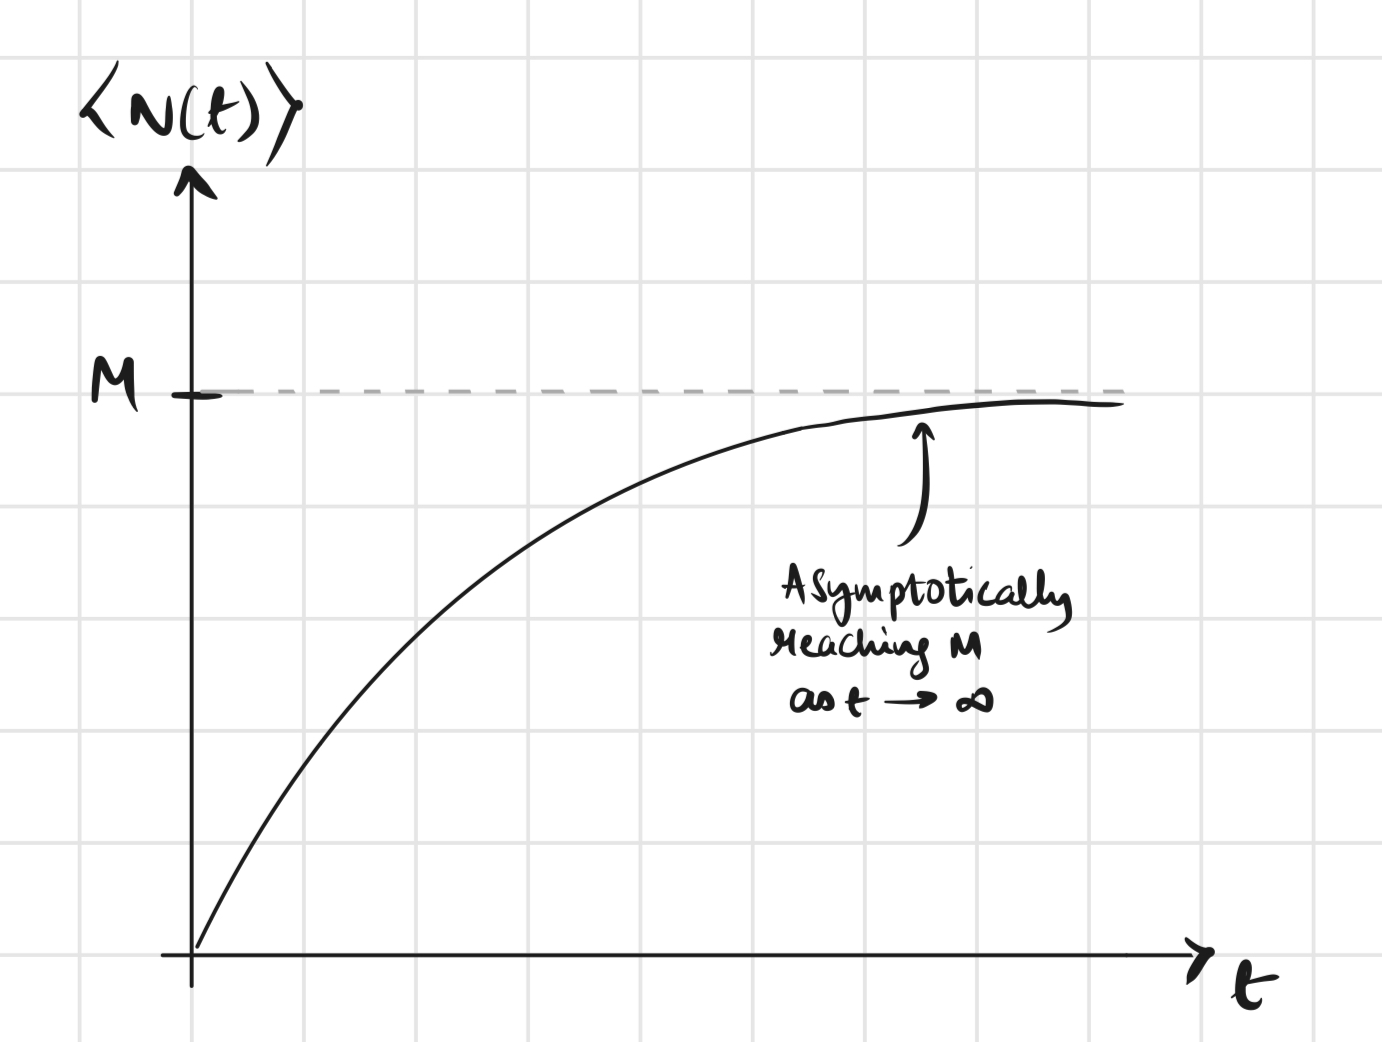
\includegraphics[width=0.6\textwidth]{figures/asymp_graph.jpg}
    \caption{\centering Graph of $\langle N(t) \rangle = M(1-e^{-\nu t})$ showing asymptotic behavior approaching $M$ as $t \to \infty$. The curve starts at origin and increases monotonically with decreasing slope.}\label{fig:asymp_graph}
\end{figure}

\newpage
\subsection*{Question 3: The tissue as a network (/37)}

\subsubsection*{a. What is the degree distribution of the cubic network when t = 1/$\nu$?}
We know from Q2b, that the probability of channel not formed at time $t$ is given by $p_0(t) = e^{-\nu t}$. As the total probability must sum to 1, we can say that the probability of a channel being formed at time $t$ is given by $p_1(t) = 1 - p_0(t) = 1 - e^{-\nu t}$. Thus, at $t = 1/\nu$, we have:

\[
    p_1(1/\nu) = 1 - e^{-1} \approx 0.632
\]

The number of channels connected to a node (its degree) here ranges from 0 to
6. Since every event is independent, this follows a binomial distribution where
probability of success is $1-e^{-1}$ and probability of failure is $e^{-1}$ and
the number of trials is 6.

\begin{equation}
    \boxed{P(X = k, t = 1/\nu) = \binom{6}{k} {(1-e^{-1})}^k {(e^{-1})}^{6-k}}
\end{equation}

\begin{align*}
    P(0) = {(e^{-1})}^6 \approx 0.002479                 \\
    P(1) = 6(1-e^{-1}){(e^{-1})}^5 \approx 0.025534      \\
    P(2) = 15{(1-e^{-1})}^2{(e^{-1})}^4 \approx 0.109714 \\
    P(3) = 20{(1-e^{-1})}^3{(e^{-1})}^3 \approx 0.251452 \\
    P(4) = 15{(1-e^{-1})}^4{(e^{-1})}^2 \approx 0.323747 \\
    P(5) = 6{(1-e^{-1})}^5{(e^{-1})} \approx 0.222409    \\
    P(6) = {(1-e^{-1})}^6 \approx 0.063665
\end{align*}

\newpage
\subsubsection*{b. Matlab Question 1}

\begin{figure}[htbp]
    \centering
    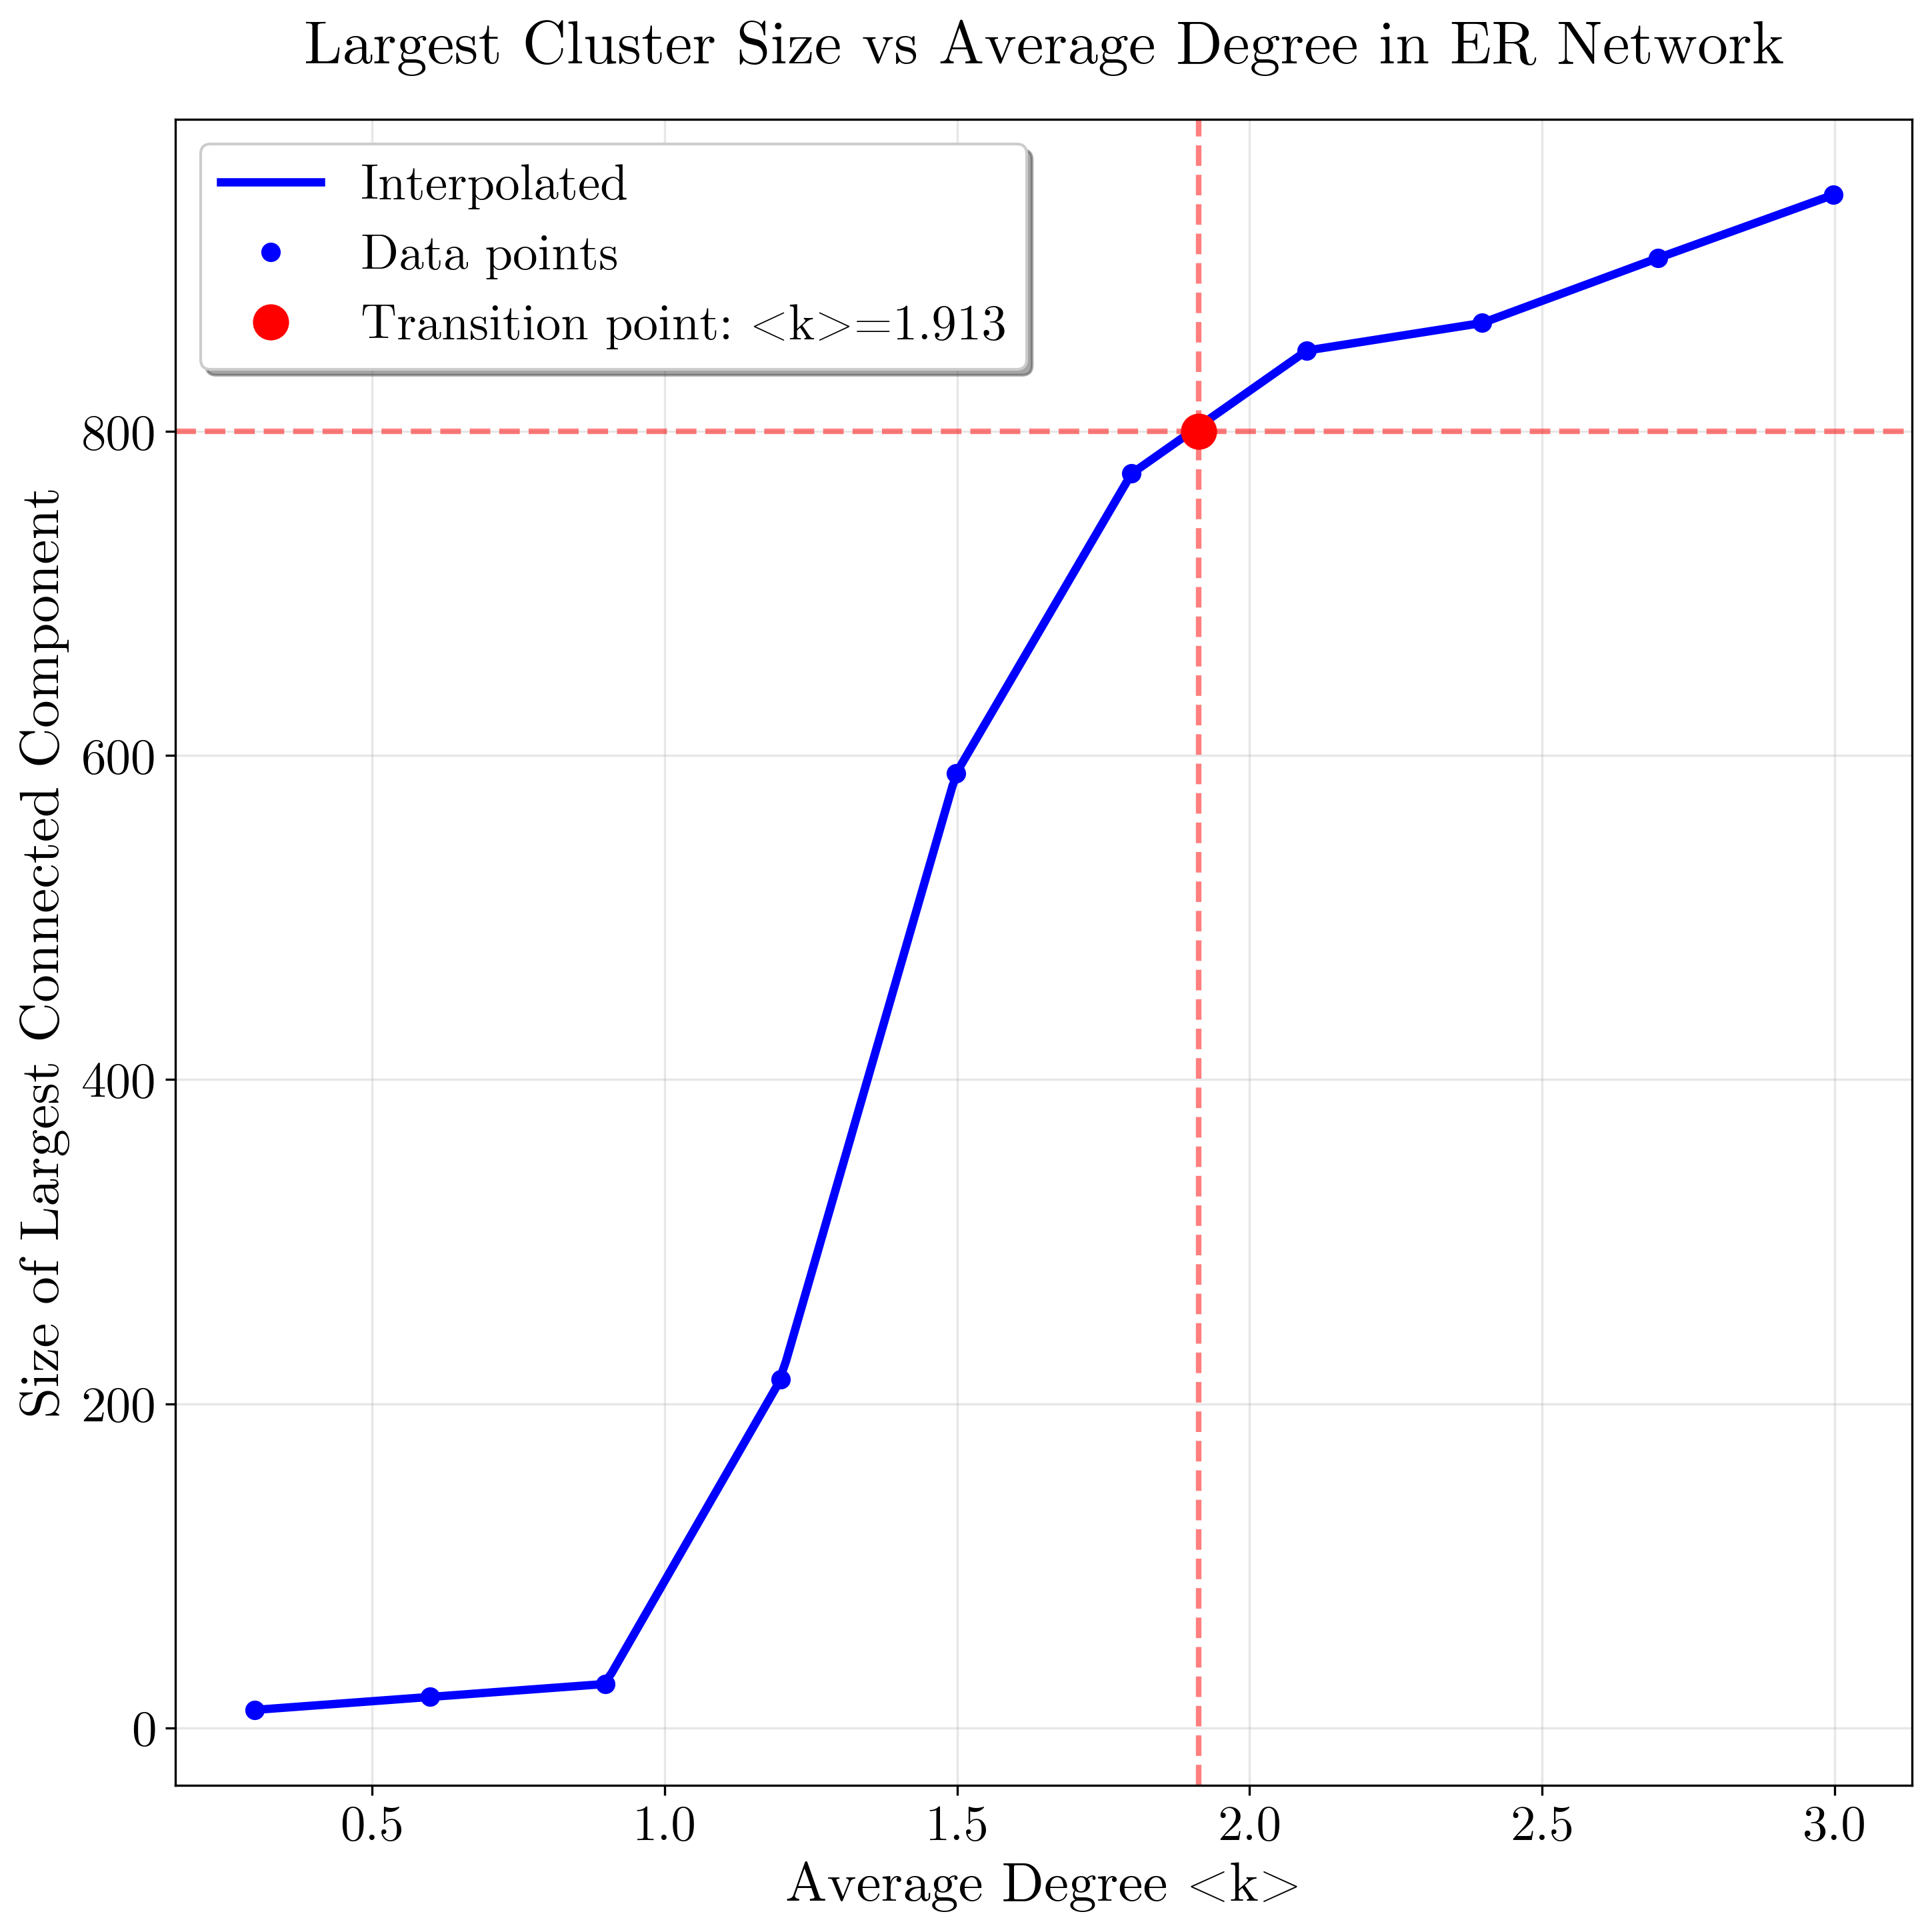
\includegraphics[width=0.7\textwidth]{figures/3b.png}
    \caption{\centering Size of largest connected component vs average node degree in an Erdős-Rényi network. A phase transition occurs near the critical degree, showing emergence of a giant component.}\label{fig:3b}
\end{figure}

The following Python code was used to generate the plot in Figure~\ref{fig:3b}:

\begin{lstlisting}[caption=Erdős-Rényi Network Analysis]
import numpy as np
# networkx library is required for this code
import networkx as nx
import matplotlib.pyplot as plt
from scipy.interpolate import interp1d

# Set font family and sizes for better quality
plt.rcParams.update(
    {
        "font.family": "CMU Serif",
        "font.size": 18,
        "axes.labelsize": 20,
        "axes.titlesize": 22,
        "xtick.labelsize": 18,
        "ytick.labelsize": 18,
        "legend.fontsize": 18,
    }
)

# Parameters
N = 1000
p_values = np.linspace(0.0003, 0.003, 10) 
avg_degree = p_values * (N - 1)
largest_cluster_sizes = []

# Simulate ER graph for each p
for p in p_values:
    A = np.triu(np.random.rand(N, N) < p, 1)
    A = A + A.T
    G = nx.from_numpy_array(A)
    largest_cluster_sizes.append(max(len(c) for c in nx.connected_components(G)))

# Create interpolation function
f = interp1d(avg_degree, largest_cluster_sizes, kind='linear')

# Create finer x points for smoother curve
x_smooth = np.linspace(min(avg_degree), max(avg_degree), 200)
y_smooth = f(x_smooth)

# Find transition point at 80% threshold using interpolated values
threshold = 0.8 * N
k_transition = x_smooth[next(i for i, size in enumerate(y_smooth) if size >= threshold)]

# Create high quality figure
plt.figure(figsize=(10, 10), dpi=300)
plt.plot(x_smooth, y_smooth, 'b-', linewidth=3, label='Interpolated')
plt.plot(avg_degree, largest_cluster_sizes, 'b.', markersize=12, label='Data points')
plt.axvline(x=k_transition, color="r", linestyle="--", alpha=0.5, linewidth=2)
plt.axhline(y=threshold, color="r", linestyle="--", alpha=0.5, linewidth=2)
plt.plot(
    k_transition,
    threshold,
    "ro",
    markersize=12,
    label=f"Transition point: <k>={k_transition:.3f}",
)

plt.xlabel("Average Degree <k>", fontweight="bold")
plt.ylabel("Size of Largest Connected Component", fontweight="bold")
plt.title("Largest Cluster Size vs Average Degree in ER Network", pad=20)
plt.grid(True, alpha=0.3)
plt.legend(frameon=True, fancybox=True, shadow=True)

# Add padding to prevent label cutoff
plt.tight_layout()
plt.show()
\end{lstlisting}

The code simulates an Erdős-Rényi network with 1000 nodes across various
probability values. It calculates the size of the largest connected component
for each probability and plots this against the average degree. The transition
point where the largest component reaches 80\% of the network size is
identified.

\newpage
\subsubsection*{c. Matlab Question 2}
\begin{figure}[htbp]
    \centering
    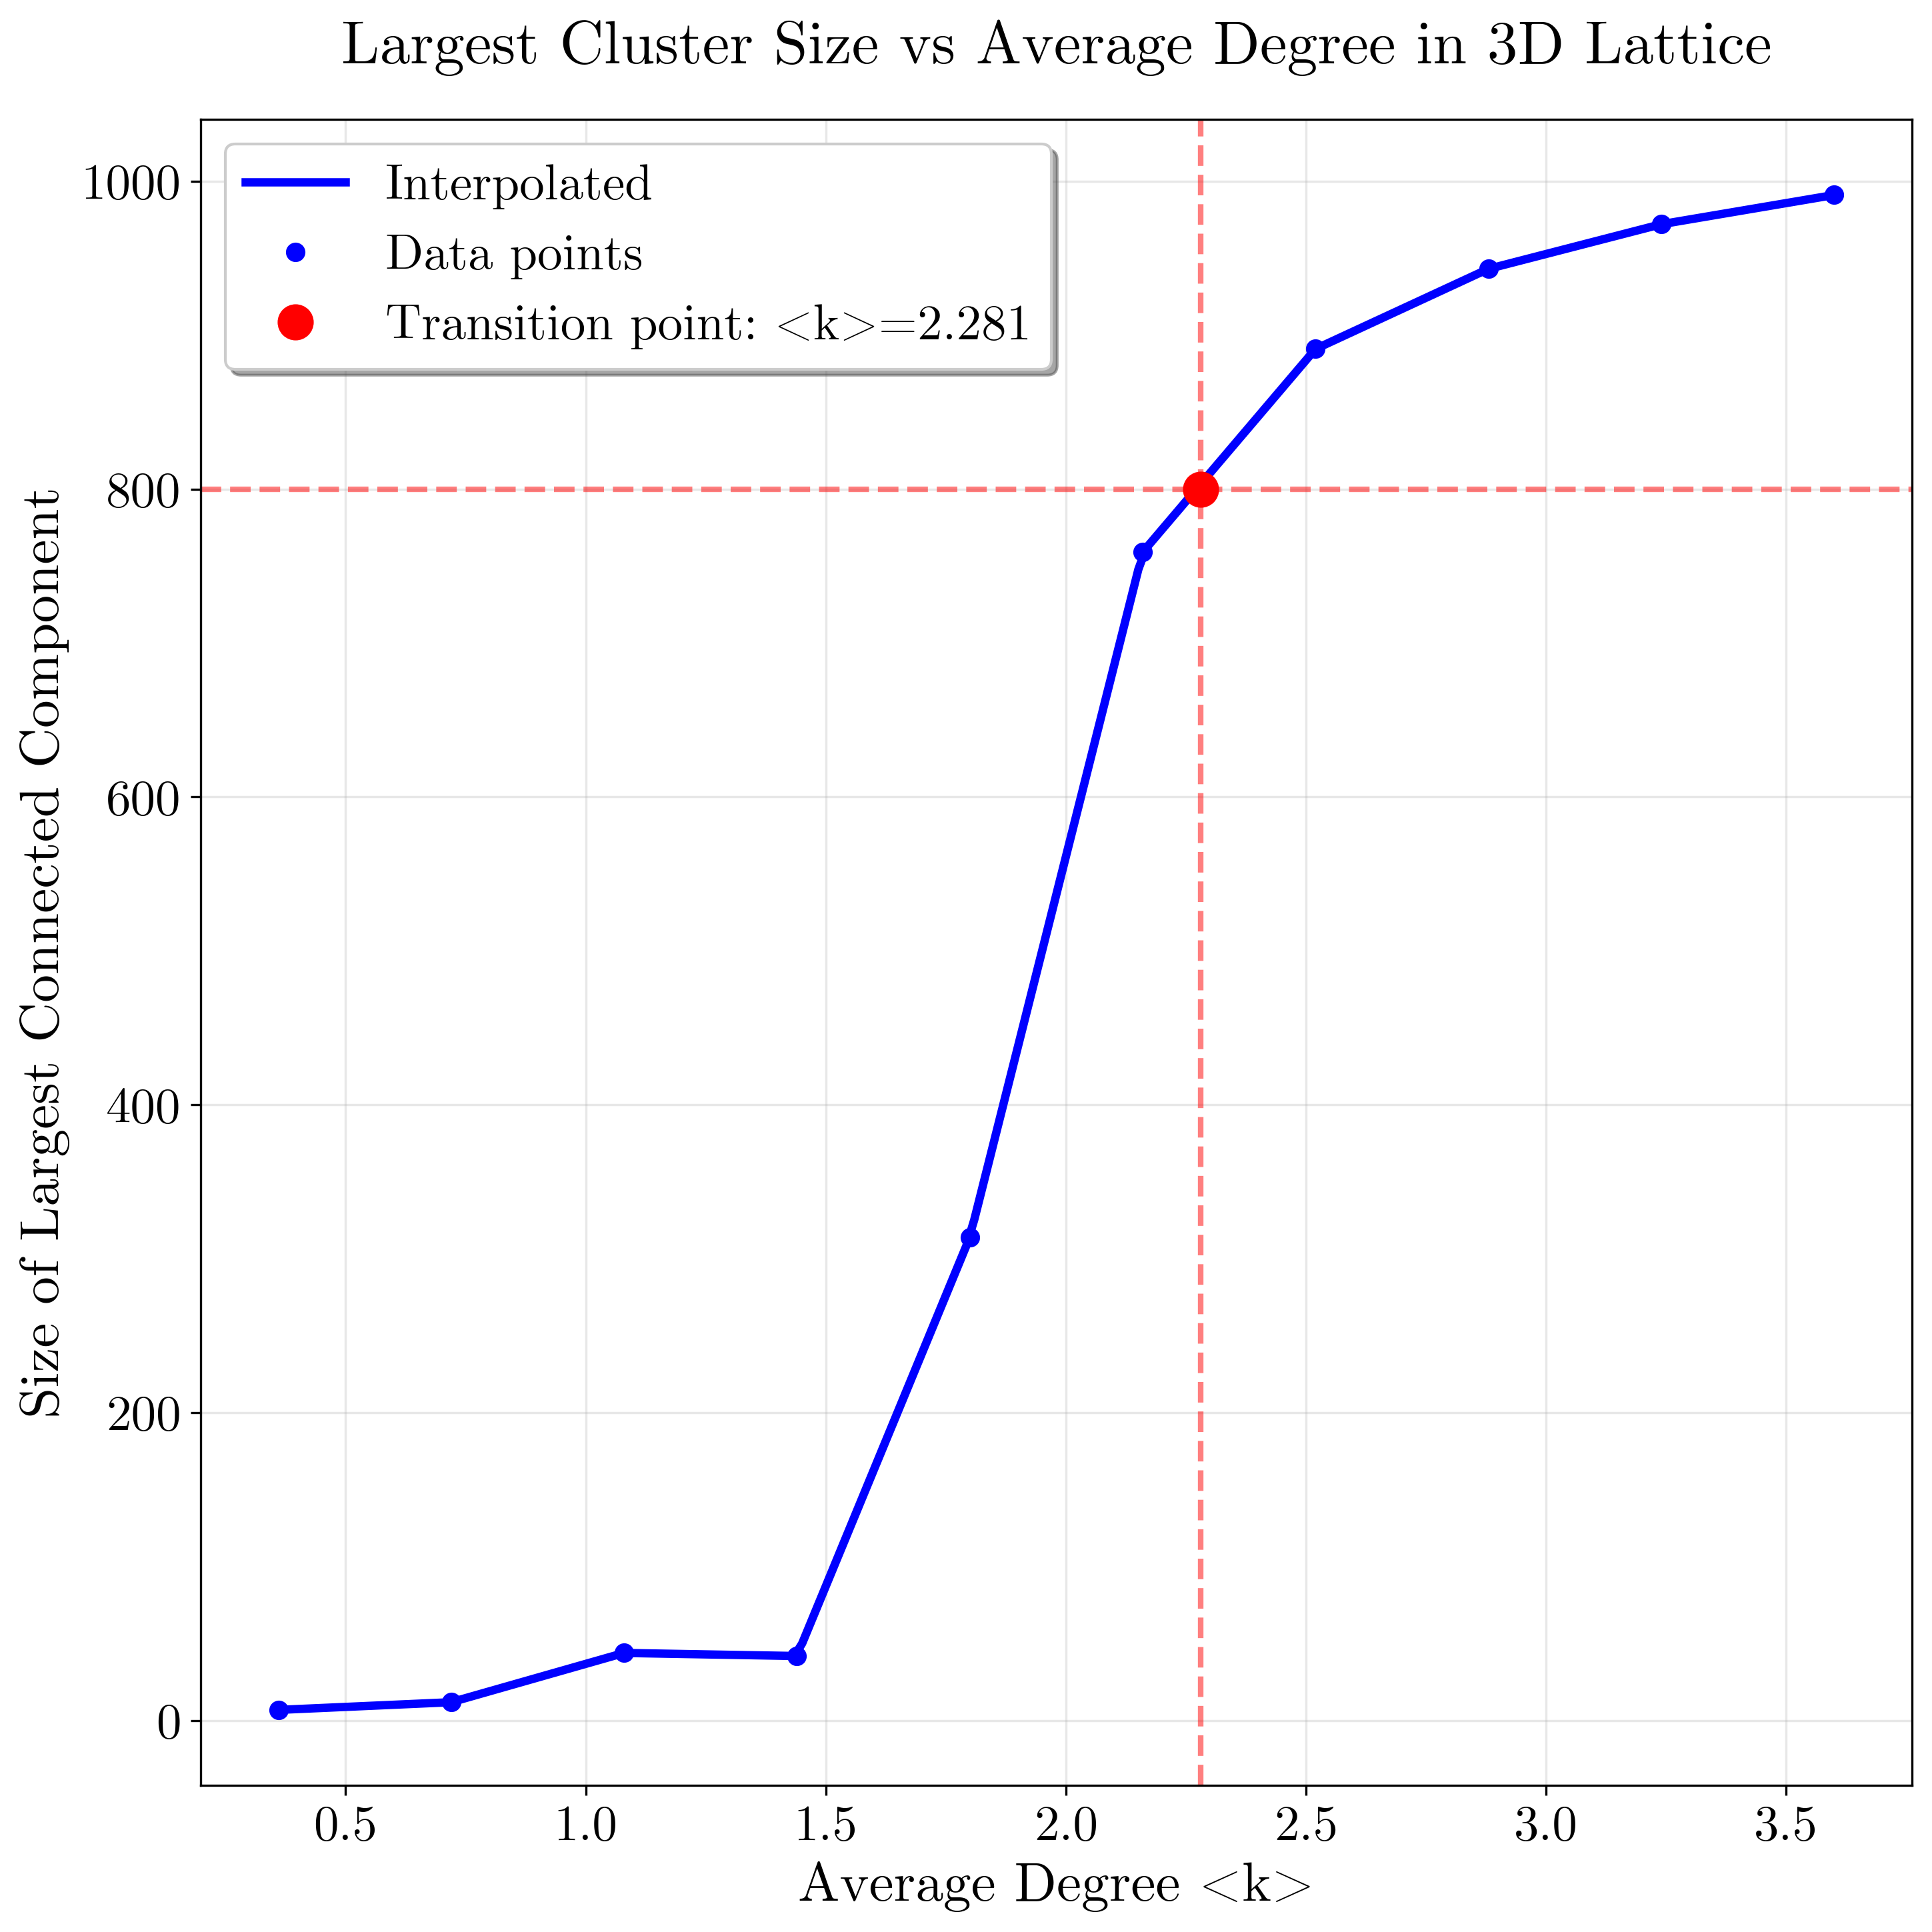
\includegraphics[width=0.7\textwidth]{figures/3c.png}
    \caption{\centering Percolation in a $10 \times 10 \times 10$ Cubic Lattice: Largest Cluster Size vs. Average Degree with Nearest-Neighbor Connections}\label{fig:3c}
\end{figure}

The following Python code was used to generate the plot in Figure~\ref{fig:3c}:

\begin{lstlisting}[caption=Cubic Lattice Percolation Analysis]
# CODE INDEPENDENT OF 3.B for Reproducibility
import numpy as np
import networkx as nx
import matplotlib.pyplot as plt
from scipy.interpolate import interp1d

# Set font sizes and DPI for high-quality output
plt.rcParams.update(
    {
        "font.family": "CMU Serif",
        "font.size": 18,
        "axes.labelsize": 20,
        "axes.titlesize": 22,
        "xtick.labelsize": 18,
        "ytick.labelsize": 18,
        "legend.fontsize": 18,
    }
)

# Parameters
N = 1000  # 10x10x10 lattice = 1000 nodes
dims = (10, 10, 10)
p_values = np.arange(0.06, 0.61, 0.06)  # 0.06 to 0.6, step 0.06
avg_degree = 6 * p_values  # Max 6 neighbors in 3D lattice
largest_cluster_sizes = []


# Function to convert 3D coordinates to node index
def xyz_to_index(x, y, z):
    return 100 * x + 10 * y + z


# Simulate cubic lattice for each p
for p in p_values:
    G = nx.grid_graph(dim=dims)  # 10x10x10 lattice
    # Remove edges randomly: keep with probability p
    edges_to_remove = [(u, v) for u, v in G.edges() if np.random.rand() > p]
    G.remove_edges_from(edges_to_remove)
    largest_cluster_sizes.append(max(len(c) for c in nx.connected_components(G)))

# Interpolation for smoother curve
f = interp1d(avg_degree, largest_cluster_sizes, kind="linear")
x_smooth = np.linspace(min(avg_degree), max(avg_degree), 200)
y_smooth = f(x_smooth)

# Find <k> at 80% threshold (800 nodes)
threshold = 0.8 * N
k_transition = x_smooth[next(i for i, size in enumerate(y_smooth) if size >= threshold)]

# Plot
plt.figure(figsize=(10, 10), dpi=300)
plt.plot(x_smooth, y_smooth, "b-", linewidth=3, label="Interpolated")
plt.plot(avg_degree, largest_cluster_sizes, "b.", markersize=12, label="Data points")
plt.axvline(x=k_transition, color="r", linestyle="--", alpha=0.5, linewidth=2)
plt.axhline(y=threshold, color="r", linestyle="--", alpha=0.5, linewidth=2)
plt.plot(
    k_transition,
    threshold,
    "ro",
    markersize=12,
    label=f"Transition point: <k>={k_transition:.3f}",
)

plt.xlabel("Average Degree <k>", fontweight="bold")
plt.ylabel("Size of Largest Connected Component", fontweight="bold")
plt.title("Largest Cluster Size vs Average Degree in 3D Lattice", pad=20)
plt.grid(True, alpha=0.3)
plt.legend(frameon=True, fancybox=True, shadow=True)
plt.tight_layout()
plt.show()
\end{lstlisting}
\end{document}